\chapter{Data structures for Fortune's algorithm}

During the algorithm we will need three data structures:
\begin{itemize}
    \item A \textbf{priority queue} $\mathcal{Q}$ for keeping track of the site and circle events.
    \item A \textbf{doubly-connected edge list (DCEL)} $\mathcal{D}$ for keeping track of the current state of the Voronoi diagram. See Definition \ref{defn:dcel}. This will be updated after each site and circle event.
    \item A self-balancing \textbf{binary search tree (BST)} $\mathcal{T}$ for keeping track of the breakpoints and arcs on the beach line.
\end{itemize}
We explain them in detail in the next sections.

\section{Priority queue}
The priority queue stores the site and circle events, and enables the algorithm to handle them in order. Each element in the priority queue has a priority. For a site event the $y$-value of the point describes the priority, and for a circle event the priority is given by the $y$-value of the lowest point of the center of the circle which describes the event. Site events also store a pointer to the site, and circle events also store the center of its definining circle and a pointer to the arc in $\mathcal{T}$ which is disappearing.

For the implementation of the priority queue we will use a binary heap. These are described in CLRS \todo{Ref}, and the implementation has been taken from \todo{Ref}.

\section{Binary search tree}

\todo{Describe how we insert into the tree at a site event}

\todo{Describe how we delete from the tree at a circle event}

\section{Doubly-connected edge list}

\todo{Describe how we modify the DCEL at a site event}

\todo{Describe how we modify the DCEL at a circle event}

\todo{Describe how we intersect the DCEL with a bounding box when we have been through the event queue}

\newpage
\section{Using a treap as the binary search tree}
In this section we will introduce the treap data structure, which is a randomized self-balancing binary search tree. The presentation follows the paper \todo{Ref}, but only describes the things that we will need.

\begin{defn}[Treap]
Let $T$ be a tree where each node $x \in T$ has properties
\begin{itemize}
    \item $x\textsf{.left}$ is the left subtree of $x$,
    \item $x\textsf{.right}$ is the right subtree of $x$,
    \item $x\textsf{.key} \in \R$,
    \item $x\textsf{.priority} \in [0,1]$.
\end{itemize}
We say that $T$ is a \textit{treap} if
\begin{enumerate}[(i)]
    \item $T$ is a binary tree with respect to $\textsf{.key}$. That is, for every $x \in T$ we have
    \begin{align*}
        \forall y \in x\textsf{.left} &\colon y\textsf{.key} \leq x\textsf{.key}, \\
        \forall y \in x\textsf{.right} &\colon y\textsf{.key} \geq x\textsf{.key}.
    \end{align*}
    \item $T$ is a max-heap with respect to $\textsf{.priority}$, that is for each $x, y \in T$:
    \begin{align*}
        x \text{ is the parent of } y \implies x\textsf{.priority} \geq y\textsf{.priority}.
    \end{align*}
\end{enumerate}
\end{defn}

\begin{defn}[Left and right rotations]
Given a tree $T$ and two nodes $x, y \in T$ with subtrees $A, B, C$ the operations \textit{rotate left} and \textit{rotate right} are given as follows:
\[
    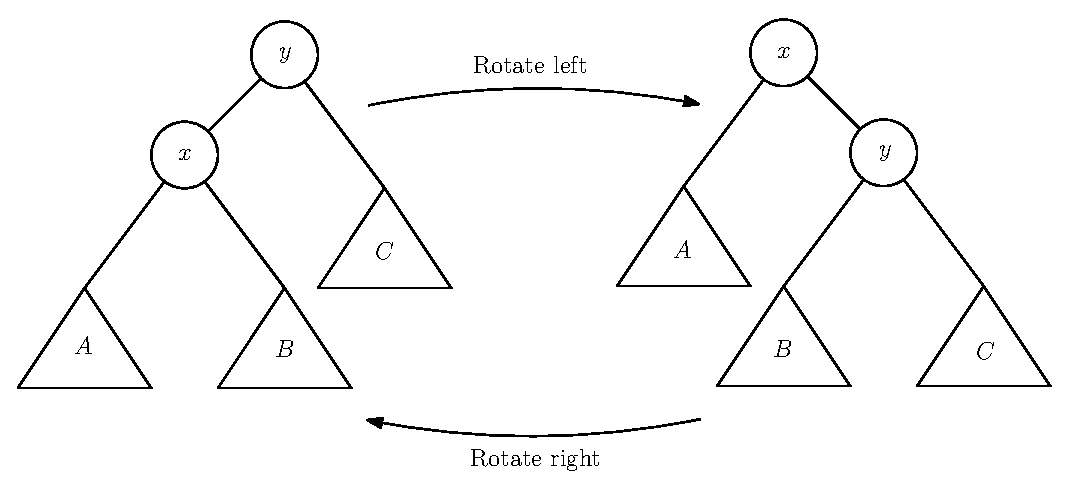
\includegraphics[width=\textwidth]{images/rotate}
\]
\end{defn}

From the diagram it is immediate that rotations preserve the binary tree property, but if $T$ has a $\textsf{.priority}$ property then the order on $x\textsf{.priority}$ and $y\textsf{.priority}$ is reversed. Given a binary tree $T$ with priorities we may then make sure it also has the max-heap property by making a finite sequence of left and right rotations, and thus we may turn it into a treap.

The basic operations on a treap are as follows:
\begin{itemize}
    \item $\textsc{Search}(x)$: This is the same as for a binary tree.
    \item $\textsc{Insert}(x)$: At first the insertion is identical to that of a binary tree: first we search for a spot to insert the new element, such that it stays a binary tree after insertion. Once inserted however, it may be the case that the max-heap property is violated. To remedy this, we may rotate $x$ up in the tree until the max-heap property is reestablished, or until we reach the root.
    \item $\textsc{Delete}(x)$: The strategy is to rotate $x$ down until it becomes a leaf in a manner which preserves the property that every subtree is a treap, and then we remove the leaf. This is done as follows: when rotating down we have a choice of rotating $x$ with the root $y$ of the left subtree $A$, or the root $z$ of the right subtree $B$. We choose to rotate $x$ and $y$ if $y\textsf{.priority} > z\textsf{.priority}$, otherwise we rotate $x$ and $z$, and then it follows by recursion that the treap property eventually is preserved in the entire tree once $x$ is a leaf, and then we clip away $x$.
\end{itemize}

\begin{defn}[Randomized search tree]
We define a \textit{randomized search tree} to be a treap $T$ where the priorities are independent, identically distributed continuous random variables.
\end{defn}

The main result we will work towards in this section is the following:

\begin{thm}
A randomized search tree storing $n$ items has the expected performance characteristics listed in the table below:
\begin{table}[h!]
\centering
\begin{tabular}{ll}
\textbf{Performance measure}   & \textbf{Bound on expectation} \\ \hline
Search                         & $\mathcal{O}(\log n)$         \\
Insertion                      & $\mathcal{O}(\log n)$         \\
Deletion                       & $\mathcal{O}(\log n)$         \\
Number of rotations per update & $\leq 2$                      \\ \hline
\end{tabular}
\end{table}
\end{thm}
To prove this we will introduce some random variables and then we will work towards proving upper bounds for their expectations. The first random variables we introduce are:
\begin{itemize}
    \item $D(x)$: the number of nodes on the path from $x$ to the root.
    \item $SL(x)$ and $SR(x)$: the length of the right spine of the left subtree of $x$ and the length of the right spine of the right subtree of $x$. By left spine of a tree we mean the number of nodes passed if we keep following the left pointer, and similarly for the right spine.
\end{itemize}
Throughout this section we will deal with a treap $T$ with nodes $x_1, x_2, \ldots, x_n$ where node $x_i$ has associated key $k_i$ and priority $p_i$, and $k_1 < k_2 < \cdots < k_n$. We now introduce the following indicator random variables:
\begin{align*}
    A_{i,j} &= \begin{cases}
        1 & \text{if } x_i \text{ is an ancestor of } x_j \text{ in } T, \\
        0 & \text{otherwise.}
    \end{cases} \\
    C_{i;\ell,m} &= \begin{cases}
        1 & \text{if } x_i \text{ is a common ancestor of } x_{\ell} \text{ and } x_{m} \text{ in } T, \\
        0 & \text{otherwise.}
    \end{cases}
\end{align*}
Note that we consider each node an ancestor of itself. We then have:
\begin{thm}
    Let $1 \leq \ell \leq n$. Then
    \begin{enumerate}[(i)]
        \item $D(x_{\ell}) = \sum_{i=1}^{n} A_{i,\ell}$.
        \item $SL(x_{\ell}) = \sum_{i=1}^{\ell-1} (A_{i,\ell-1} - C_{i;\ell-1,\ell})$.
        \item $SR(x_{\ell}) = \sum_{i=\ell+1}^{n} (A_{i,\ell+1} - C_{i;\ell,\ell+1})$.
    \end{enumerate}
\end{thm}
\begin{proof}
\todo{.}
\end{proof}

If we let $a_{i,j} = \mathbb{E}[A_{i,j}]$ and $c_{i;\ell,m} = \mathbb{E}[C_{i;\ell,m}]$ then by linearity of expectation we get:
\begin{cor}
Let $1 \leq \ell \leq n$ and let $\ell < m$. Then
    \begin{enumerate}[(i)]
        \item $\mathbb{E}[D(x_{\ell})] = \sum_{i=1}^{n} a_{i,\ell}$.
        \item $\mathbb{E}[SL(x_{\ell})] = \sum_{i=1}^{\ell-1} (a_{i,\ell-1} - c_{i;\ell-1,\ell})$.
        \item $\mathbb{E}[SR(x_{\ell})] = \sum_{i=\ell+1}^{n} (a_{i,\ell+1} - c_{i;\ell,\ell+1})$.
    \end{enumerate}
\end{cor}

Our analysis has now been reduced to determining the expectations $a_{i,j}$ and $c_{i;\ell,m}$. Now, if $X$ is an indicator random variable, then
\[
    \mathbb{E}[X] = \textsf{Pr}(X = 1),
\]
so we get that
\[
    a_{i,j} = \textsf{Pr}(A_{i,j} = 1) = \textsf{Pr}(x_i \text{ is an ancestor of } x_j)
\]
and
\[
    c_{i;\ell,m} = \textsf{Pr}(C_{i;\ell,m} = 1) = \textsf{Pr}(x_i \text{ is a common ancestor of } x_{\ell} \text{ and } x_{m}).
\]
Determining these probabilities is made possible through the ancestor lemma:
\begin{lem}[Ancestor lemma]
Assuming all priorities are distinct, then $x_i$ is an ancestor of $x_j$ in $T$ if and only if $p_i \geq p_h$ for all $i \leq h \leq j$.
\end{lem}
\begin{proof}
\todo{.}
\end{proof}

\newpage
\begin{thm}
Let $1 \leq \ell \leq m$. In a randomized search tree with $n$ nodes the following expectations hold:
\begin{enumerate}[(i)]
    \item $\mathbb{E}[D(x_{\ell})] = H_{\ell} + H_{n+1-\ell} - 1 < 1 + 2 \cdot \ln n = \mathcal{O}(\log n)$.
    \item $\mathbb{E}[SL(x_{\ell})] = 1 - \displaystyle \frac{1}{\ell}$.
    \item $\mathbb{E}[SR(x_{\ell})] = 1 - \displaystyle \frac{1}{n + 1 - \ell}$.
\end{enumerate}
\end{thm}
\begin{proof}
For (i) we get
\begin{align*}
    \mathbb{E}[D(x_{\ell})] &= \sum_{i=1}^n a_{i,\ell} \\
    &= \sum_{i=1}^n \frac{1}{\abs{i - \ell} + 1} \\
    &= \sum_{i=1}^{\ell} \frac{1}{\ell - i + 1} + \sum_{i=\ell}^{n} \frac{1}{i - \ell + 1} - 1 \\
    &= \sum_{i=1}^{\ell} \frac{1}{i} + \sum_{i=1}^{n+1-\ell} \frac{1}{i} - 1 \quad \text{(Reverse left sum and swap index in right)} \\
    &= H_{\ell} + H_{n+1-\ell} - 1 \\
    &< (1 + \ln \ell) + (1 + \ln (n + 1 - \ell)) - 1 \\
    &\leq 1 + 2 \cdot \ln n.
\end{align*}
For (ii) we have
\begin{align*}
    \mathbb{E}[SL(x_{\ell})] &= \sum_{i=1}^{\ell - 1} \left(a_{i,\ell-1} - c_{i;\ell-1,\ell}\right) \\
    &= \sum_{i=1}^{\ell - 1} \left(\frac{1}{\abs{i - (\ell - 1)} + 1} - \frac{1}{\max\curly{i,\ell-1,\ell}-\min\curly{i,\ell-1,\ell}+1}\right) \\
    &= \sum_{i=1}^{\ell - 1} \left(\frac{1}{\ell - i} - \frac{1}{\ell - i + 1}\right) \\
    &= \frac{1}{\ell - (\ell - 1)} - \frac{1}{\ell} \quad \text{(The above is a telescoping sum)} \\
    &= 1 - \frac{1}{\ell}.
\end{align*}
For (iii) we note that the proof is basically the same as for (ii).
\end{proof}

\todo{Show that 2 rotations are the expected amount}